\begin{appendices}
	\chapter{Syllable classification through histogram segmentation} \label{appendix:split_syllables}
	The syllable classifiers in sections \ref{cha:exper_classifier} and \ref{cha:generalisation_study} take as input a fixed-length speech wave of a syllable. However, the words in the speech dataset are not yet split up into syllables, and we must do this ourselves.
	
	To split up the sound files in the dataset, we make use of Otsu's histogram segmentation algorithm \citep{otsuTlresholdSelectionMethod1979}. Afterwards, the split speech waves are padded with zeros in the front and back such that each wave has the same length. The files are padded to contain 8800 samples (at a sample rate of 16 kHz.).
	
	Otsu's algorithm is traditionally used for segmentation applications on greyscale images. Given an individual image, it chooses a particular intensity threshold and classifies all pixels into one of two classes depending on whether their intensity values are smaller or larger than the threshold. The threshold is chosen to be the one that minimises the intra-class variance \cite{OtsuMethod2023}. 
	
	We explore an alternative domain for the algorithm and use it to find an amplitude threshold in the speech waves. The recordings are consistent in loudness and each file contains exactly three syllables of the form ``consonant - vowel". It, therefore, suffices to find a single threshold per audio file that classifies the amplitudes as vowel or consonant.
	
	We first max pool the audio waves with a window size of 0.02 seconds. This emphasises the discrepancy in amplitude between vowels and consonants, as shown in figure \ref{fig:max sliding window}. The threshold that minimises the variance for the two classes is computed using a histogram, shown in figure \ref{fig:histogram}, in this case, 0.10. 
	
	The time windows with an amplitude smaller than 0.10 are classified as consonant, and the other time windows as vowel. However, when directly using the threshold on the max pooled speech wave we observed that not all consonants were detected, and thus too much speech wave was being classified as consonant. Instead, we found that applying the threshold (still obtained from the max pooled speech wave) to the 90'th percentile was a good compromise between classifying speech chunks as vowel or consonant. Once the vowels and consonants are obtained, syllables are computed at transition points going from vowel to consonant, shown in figure \ref{fig:full sound wave adjusted yaxis}. The transition points mark the ending of a syllable.

	Apart from a few edge cases, this technique worked well enough for our purposes. In the cases where more than three vowels were obtained, the transition points closest to the one-third and two-third duration mark were considered instead.

		
		\begin{figure}
			\centering	
			\begin{minipage}{\linewidth}
				\centering
				
				\begin{subfigure}{\linewidth}
					\centering
					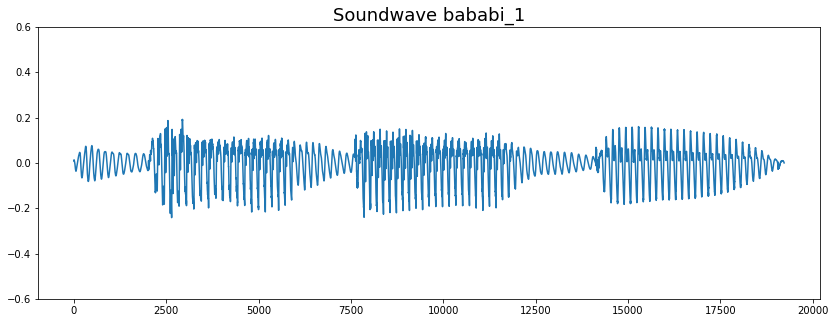
\includegraphics[width=0.5\linewidth]{screenshot017}
					\caption{Sound wave for ``ba ba bi", which should be split up into ``ba", ``ba and ``bi".}
					\label{fig:full sound wave adjusted yaxis}
				\end{subfigure}
				
				\vspace{1em}
				
				
				\begin{subfigure}{\linewidth}
					\centering
					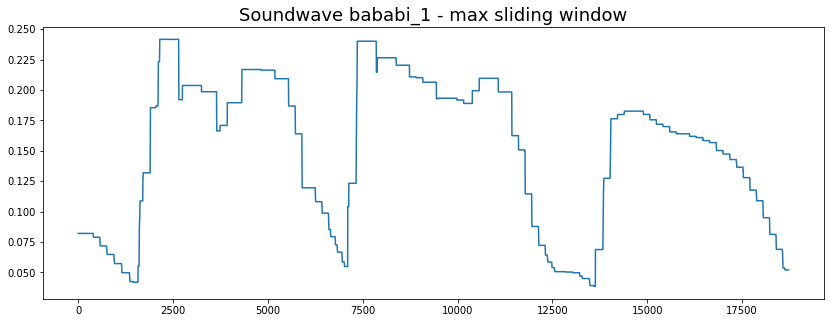
\includegraphics[width=0.5\linewidth]{screenshot012}
					\caption{Resulting speech wave after max pooling. The threshold will be computed using this speech wave.}
					\label{fig:max sliding window}
				\end{subfigure}
				
				\vspace{1em}
				
				\begin{subfigure}{\linewidth}
					\centering
					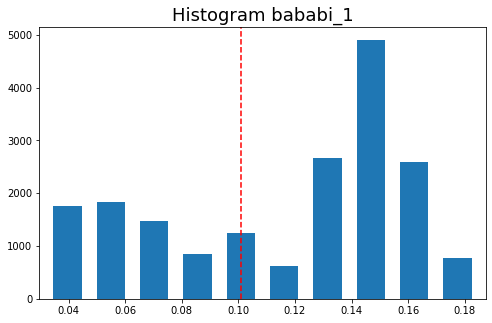
\includegraphics[width=0.3\linewidth]{screenshot018}
					\caption{Threshold obtained using Otsu's algorithm. The red dashed line corresponds to the threshold.}
					\label{fig:histogram}
				\end{subfigure}
				
				\vspace{1em}
				
				\begin{subfigure}{\linewidth}
					\centering
					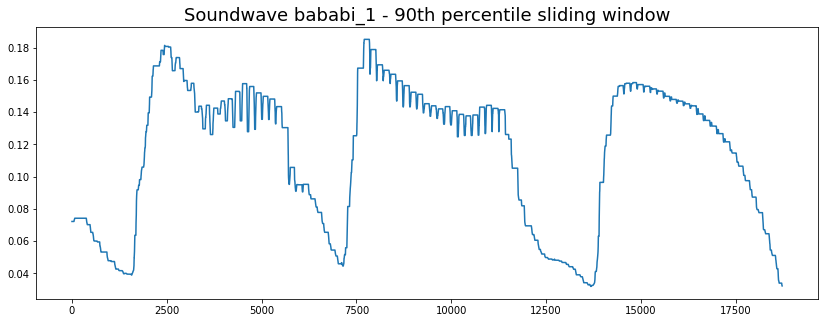
\includegraphics[width=0.5\linewidth]{screenshot013}
					\caption{90'th percentile speech wave (computed using moving window of 0.02 seconds). The threshold is applied to this speech wave. Amplitudes larger than the threshold are considered vowels and smaller values are consonants.}
					\label{fig:90th percentile}
				\end{subfigure}
			
				\vspace{1em}				
				
				\begin{subfigure}{\linewidth}
					\centering
					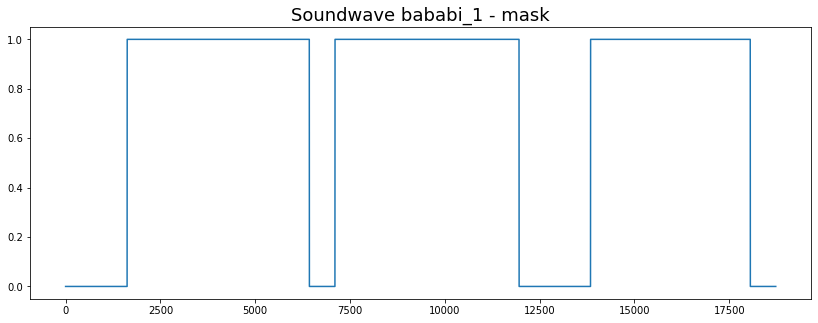
\includegraphics[width=0.5\linewidth]{screenshot014}
					\caption{Obtained mask from applying the threshold. The x coordinates going from one to zero are transition points and mark the end of a syllable. There are three potential points in this image. Since each audio file contains three syllables (and thus a maximum of two transition points), the two \textit{true} points are selected based on their distance from the one-third and two-third x coordinate. In this case, the last transition point will be discarded.}
					\label{fig:mask}
				\end{subfigure}
				
				\vspace{1em}
				
				\begin{subfigure}{\linewidth}
					\centering
					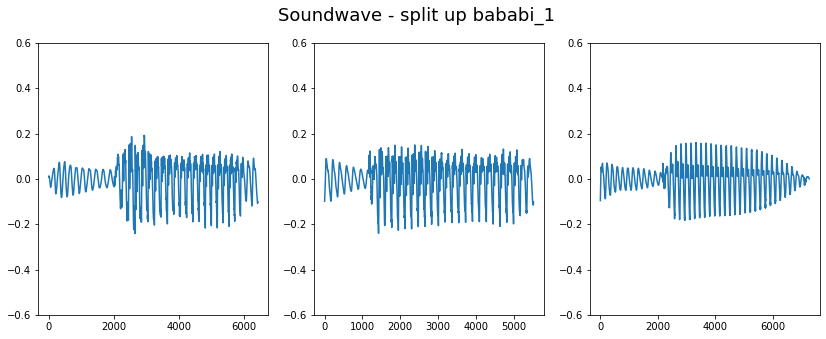
\includegraphics[width=0.5\linewidth]{screenshot016}
					\caption{The three obtained syllables after cutting the speech wave at the two transition points.}
					\label{fig:split up sound wave}
				\end{subfigure}
			\end{minipage}			
		\end{figure}
	



	




%	\section{GIM: Activation visualisations}
%	
%	%these were notes from the decoder from file: eval_autoencoder.py
%	thought for later: its actually weird i was able to play enc as audio as enc is 512 x something
%	so huh? that means that a lot of info is already in first channel? what do other 511 channels then contain?
%	"""
%	Observations:
%	First layer decoded still contains the same sound, but with some added noise (could be because decoder hasn't trained very).
%	However, the encoded first layer, still contains the exact sound as the original sound. It is however downsampled a lot -> from 16khz to ~3khz
%	"""
%	thought for later: its actually weird i was able to play enc as audio as enc is 512 x something
%	so huh? that means that a lot of info is already in first channel? what do other 511 channels then contain?
%	
%	
%	
%	\begin{figure}[h]
%		\centering
%		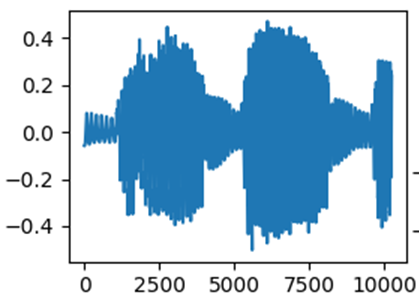
\includegraphics[width=0.7\linewidth]{screenshot007}
%		\caption{"BA-BA-BA" time domain}
%		\label{fig:screenshot007}
%	\end{figure}
%	
%	\begin{figure}[h]
%		\centering
%		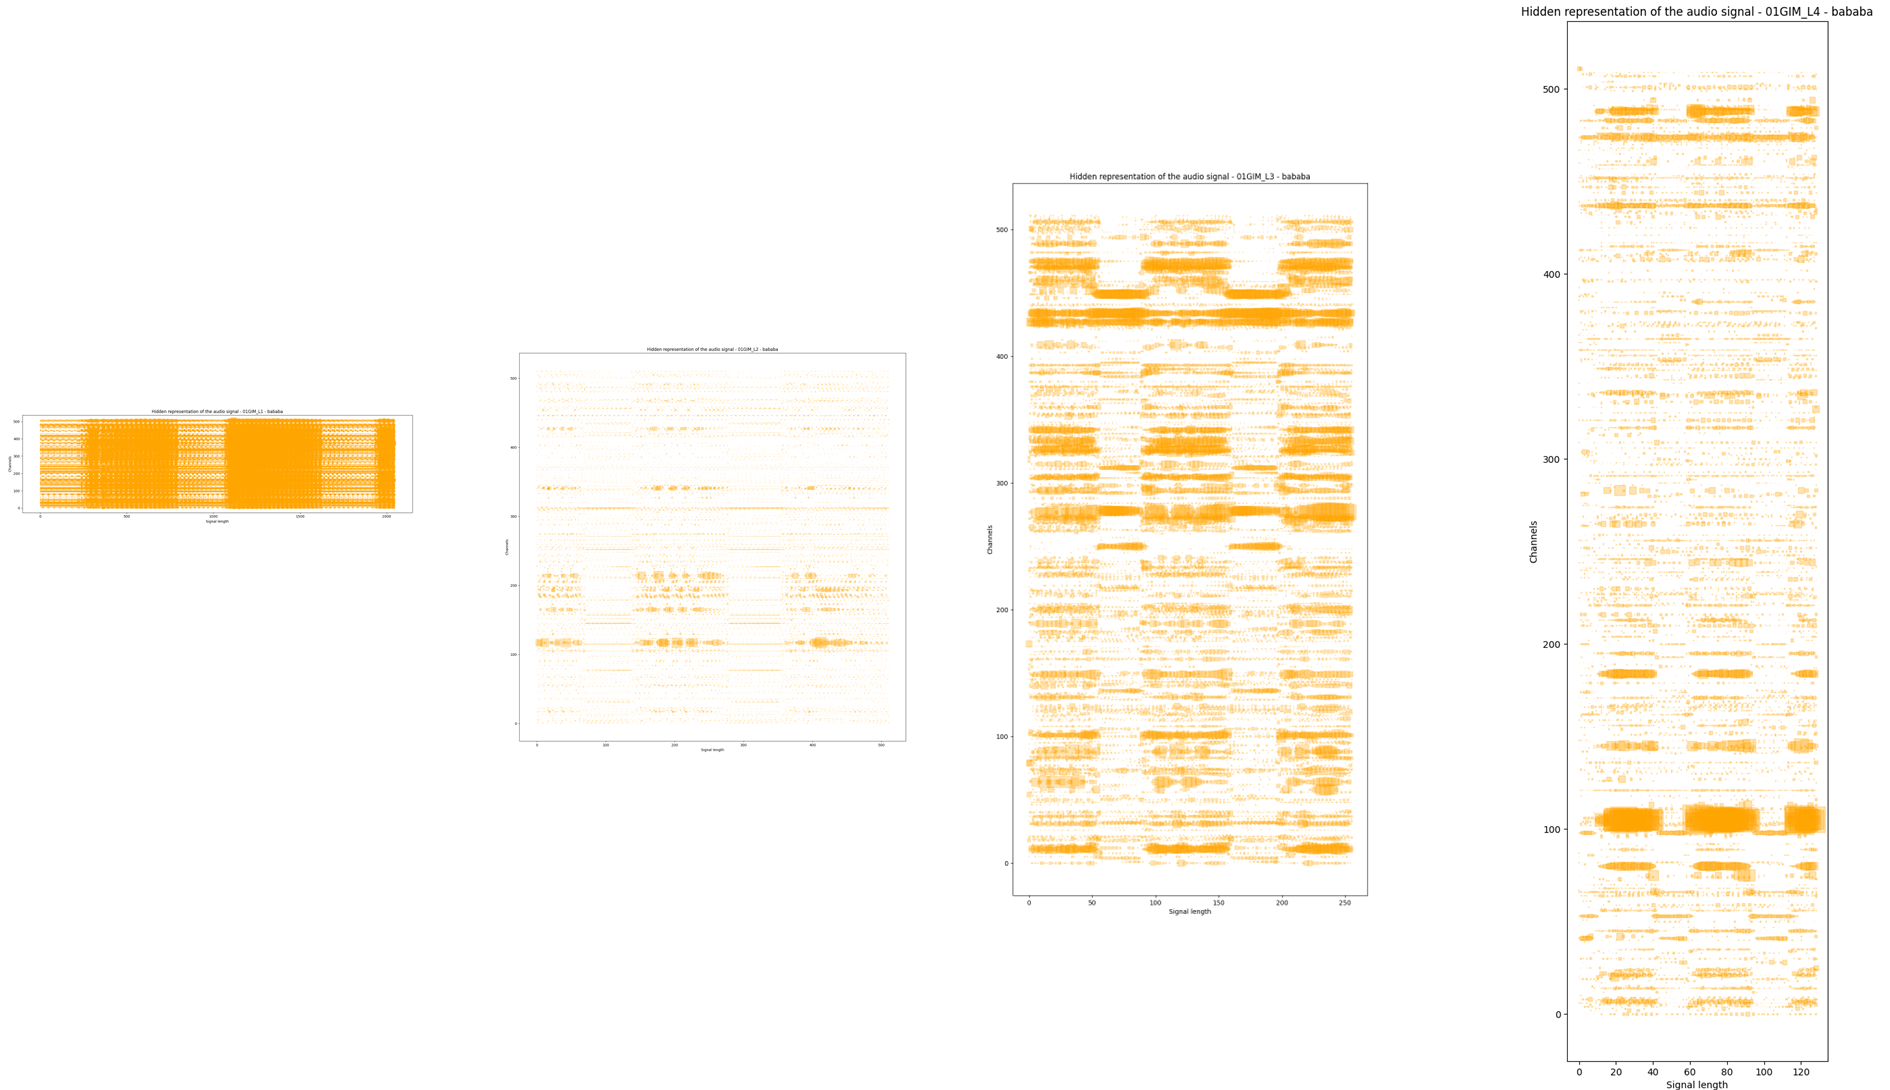
\includegraphics[width=0.7\linewidth]{screenshot006}
%		\caption{Activations of the sound "BA-BA-BA" through GIM}
%		\label{fig:gim latent activations}
%	\end{figure}
%	
%	No batch normalisation, so although channels appear to have larger activations than other channels, size of activation does not really say anything about information. eg activations 0.01 could still contain more information than 3.0 activation.
%	
%	Since the activations from convolutional neural networks, the order is still maintained. Hence, can align activations with original signal.
%	
%	Observations in latent representations:
%	
%	\textit{Layer 1:}
%	The activations of the first decoder still contain a lot of similarity with the original signal, in terms of structure. There is a lot of redundant data within the representation. Eg: the one channel could be replied 
%	
%	Layer 2
%	
%	Layer 3:
%	
%	Layer 4:
%	Still notices multiple channels which have high activations when signal is has high amplitudes and small activations when amplitude is low. 
%	
%	Also activations which are high when volume is low. --> indicates that certain kernel weights are sensitive for \textbf{"klinkers"} and other kernels for \textbf{medeklinkers}. see \ref{fig:screenshot008}.
%	
%	\begin{figure}[h]
%		\centering
%		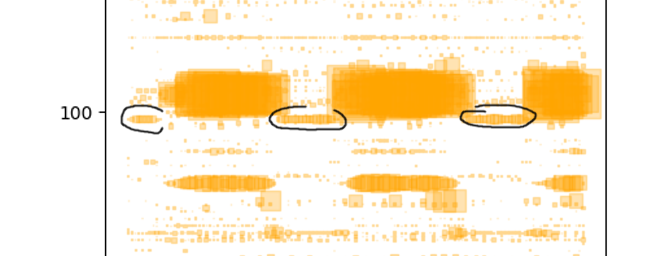
\includegraphics[width=0.7\linewidth]{screenshot008}
%		\caption{zoomed in}
%		\label{fig:screenshot008}
%	\end{figure}
%	
%	
%	Observe that activations happen in clusters/sequences. So it is usually a patch of signal samples that cause high activations. This could for instance indicate that both kernels are sensitive for the \textbf{medeklinker} "b", but sensitive for different features. eg the letter B has spoken sound "buh". so maybe one is sensitive for "b" and other for "uh".
%	
%	Figure \ref{fig:layer4 zoomed in} also nicely shows how different channels have clusters of activations at slightly different times. 
%	
%	\begin{figure}[h]
%		\centering
%		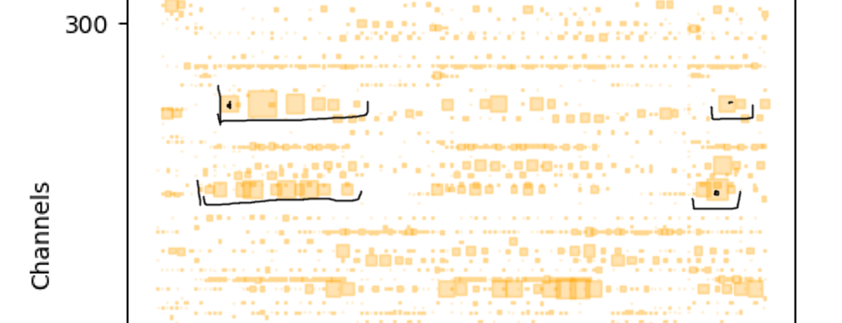
\includegraphics[width=0.7\linewidth]{screenshot010}
%		\caption{Zoomed in}
%		\label{fig:layer4 zoomed in}
%	\end{figure}
	
	

\end{appendices}